\section{Introduction}
\todo{This chapter needs citations and figure refs fixed}
\todo{This chapter also needs editing to many sections to re-frame work}
As part of the ongoing research into the growth of CdTe, various other oxide single crystals were examined for possible use as substrates. One of those substrates, SrTiO\textsubscript{3}, while it did not ultimately yield particularly high quality CdTe, did provide some interesting insights into the potential for surface reconstructions to play a role in epitaxy.

The role of both substrate offcut and high temperature surface reconstructions were examined through the growth of CdTe on as-received and reconstructed SrTiO\textsubscript{3} substrates. This work was done in close collaboration with Dr. Robert Hughes and Dr. Svetlana Neretina and was published in Applied Surface Science\cite{Neretina2009a}.

\section{Experimental}
CdTe films were deposited on both the as-received and
reconstructed surface of (100) SrTiO\textsubscript{3} (MTI Corporation). Step-
terrace formation relied upon the miscut originating from the
inaccuracies in the crystallographic alignment carried out prior to
the cutting and polishing of the substrates (manufacturer’s miscut
tolerance 0.5\degree). As a result, the degree of miscut could only be
varied through the use of substrates from different batches. Due to
the high temperatures required, the surface reconstruction took
place ex situ in a quartz tube furnace. Prior to annealing, the
substrates were etched in BHF for 90~s. Anneals were conducted in
flowing oxygen (60 cm\textsuperscript{3}/min) at 1000\degree\celsius~for 10~h. \cref{fig:srtio3_sub_afm} shows
atomic force microscopy (AFM) images for the as-received and
surface reconstructed substrates relevant to this work. As
expected, only the annealed substrates exhibit the step-terrace
structure with unit cell step heights. The difference in terrace
width for the surfaces shown in \cref{fig:srtio3_sub_afm}b and c can be attributed to a
miscut difference estimated at 0.358\degree. Also present on each image
are the crystallographic axes obtained through X-ray diffraction
(XRD). Note that a nearly identical in-plane step direction exists for
both reconstructed surfaces. As this direction is close to, but not
aligned with the [011] axis of SrTiO\textsubscript{3}, it is expected that the steps
exhibit a saw-tooth morphology, but on length scales not readily
observed using atomic force microscopy.
\begin{figure}
    \centering
    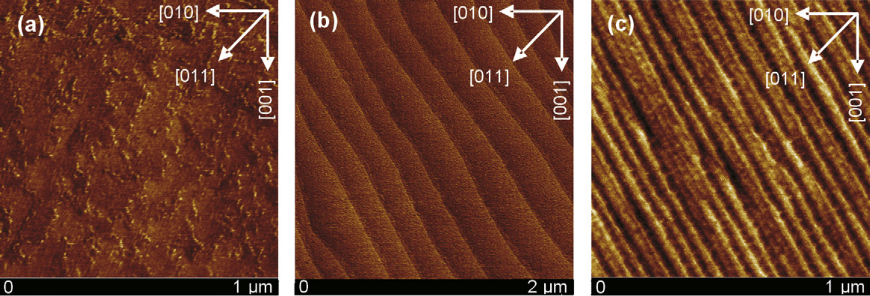
\includegraphics[width=\textwidth]{srtio3_sub_afm}
    \caption[AFM of SrTiO\textsubscript{3} surfaces]{\label{fig:srtio3_sub_afm}AFM images for the (a) as-received (100) SrTiO\textsubscript{3} substrate, (b) a reconstructed surface with an average terrace width of approximately 200 nm and (c) a reconstructed surface with a terrace width of approximately 50 nm. From the step heights and terrace widths it is estimated that the miscuts for the two reconstructed surfaces are (b) 0.118\degree{}
        and (c) 0.468\degree{}.}
\end{figure}

CdTe films were deposited on the three SrTiO\textsubscript{3} surfaces shown
in \cref{fig:srtio3_sub_afm} using pulsed laser deposition. A deposition rate of 20 nm/min was achieved by
operating the laser at a repetition rate of 10 Hz with a substrate to
target distance of 3.5 cm. Films were grown to
a thickness of 300 nm as determined using a spectroscopic variable
angle ellipsometer (Horiba Jobin Yvon, France). Morphological and
structural characterization was then conducted on the films
produced using AFM and 2DXRD.
\section{Results and Discussion}
\cref{fig:srtio3_pole} shows the (111) CdTe pole figures for the three substrates
shown in \cref{fig:srtio3_sub_afm}. The dramatic differences observed between films
deposited on the as-received and annealed substrates indicate that
the surface reconstruction gives rise to a complete re-alignment of
the CdTe grains. The pole figure for the as-received surface is
consistent with a [111] oriented film. The fact that twelve peaks
exist in the outer ring, instead of the three expected for a single
crystal, indicates that there are four in-plane grain orientations.
The pole figures for the films deposited on the surface reconstructed substrates show that both films are predominantly [211]
oriented. The twelve peaks in the central ring and twenty-four
peaks in the outer ring denote twelve in-plane grain orientations. Each peak in the central ring comes from a different grain, the intensity differences indicate that some grains form
preferentially over others. Note that of the twelve peaks both
the strongest and weakest is in-line with the miscut direction for
both of the reconstructed surfaces and that the degree of this
preferential orientation is stronger for the reconstructed surface
having the narrow terrace width. An examination of the low
intensity pole figure peaks (not visible in the figures), indicates that
some [111] CdTe grains exist in these nominally [211] films, but
at the 10\% level. While these [111] grains contribute to
the intensity at the centre of the pole, the response there is almost
entirely due to the (100) SrTiO\textsubscript{3} substrate.
\begin{figure}
    \centering
    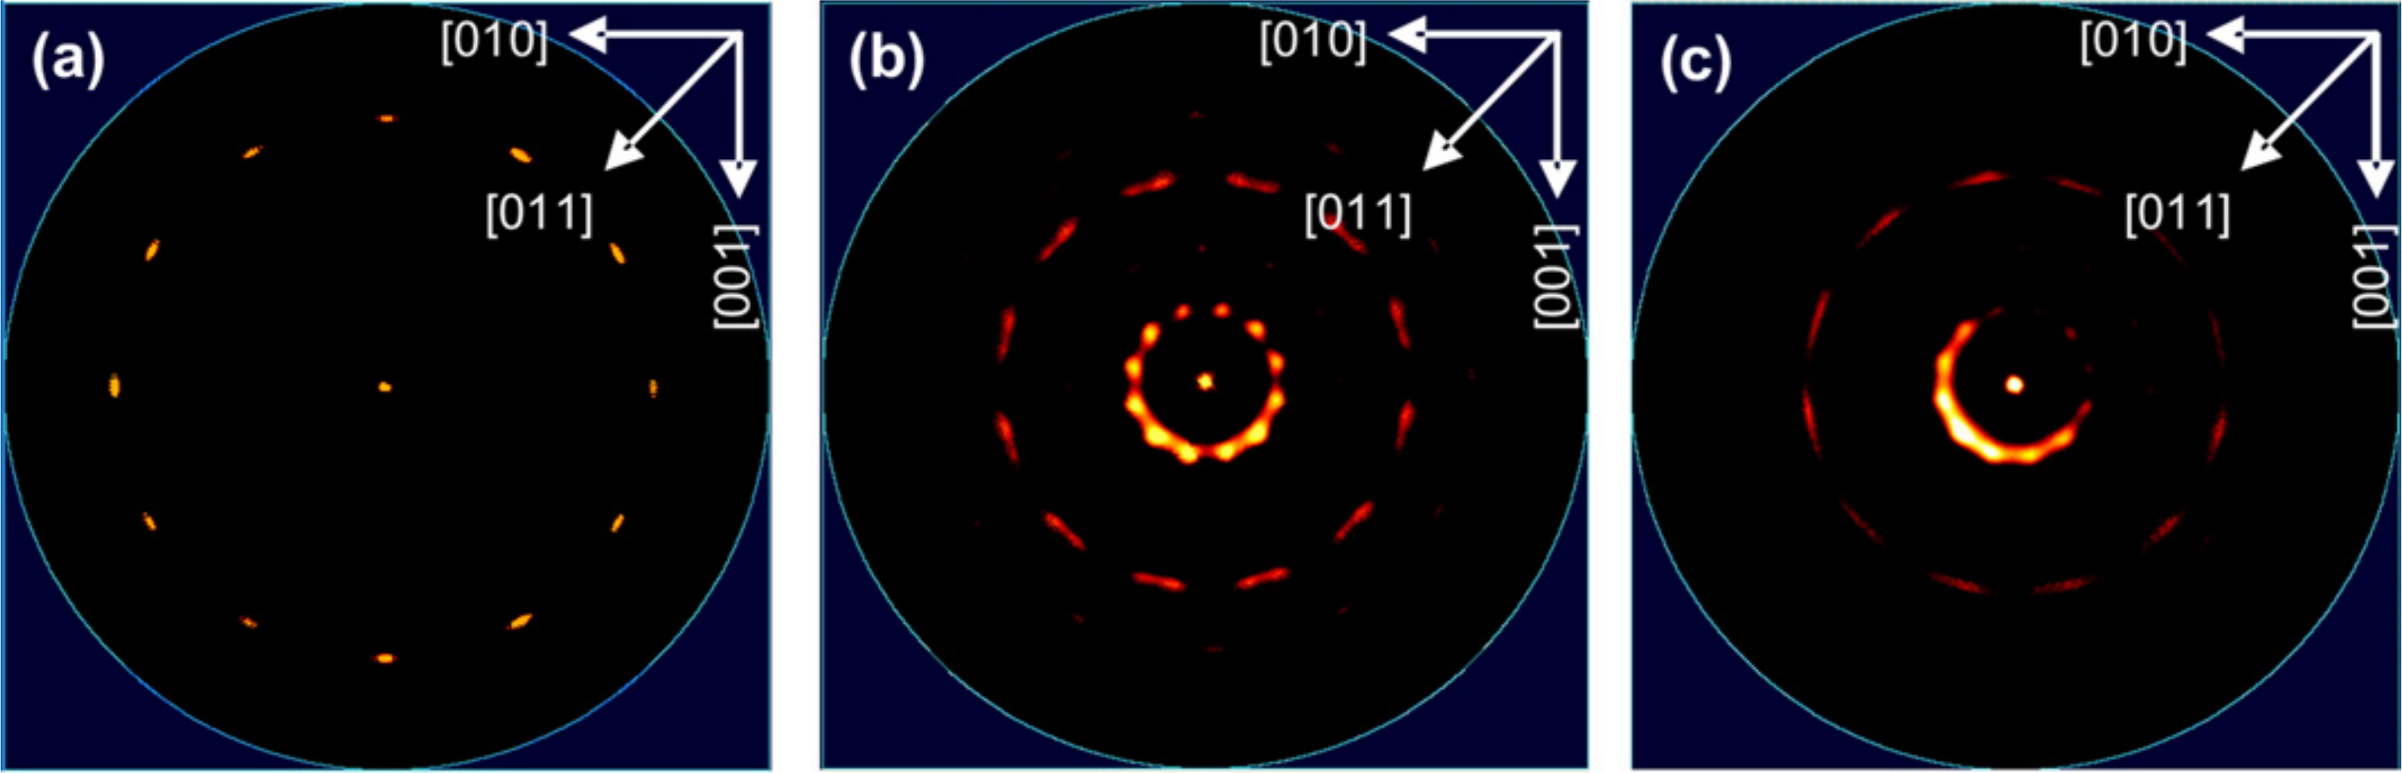
\includegraphics[width=\textwidth]{srtio3_pole}
    \caption[Pole figures of CdTe grown on SrTiO\textsubscript{3}]{\label{fig:srtio3_pole}(111) CdTe pole figures for films deposited on (a) the as-received (100) SrTiO\textsubscript{3} substrate (b) the reconstructed surface with wide terraces and (c) the reconstructed surface with narrow terraces. Indicated on each image are the substrate’s in-plane crystallographic axes obtained from XRD measurements.}
\end{figure}
Grain formation for a given film/substrate combination is
determined by the interface energy. For the case of the as-received
(100) SrTiO\textsubscript{3} substrate the interface energy is minimized through
the formation of [111] CdTe grains. This interfacial relationship is
not surprising as CdTe has demonstrated a high propensity for
forming it almost irrespective of the substrate surface offered\cite{Neretina2006}.
The resulting interface, however, must overcome the seemingly
incompatible situation brought about when the four-fold symmetric substrate surface mates with the six-fold symmetric (111)
plane of CdTe. In this scenario it is reasonable to expect that the
resulting in-plane grain structure reflects both a suitable fit to the
substrate’s atomic arrangement as well as its underlying symmetry. The (111) pole figure results indicate that this is indeed the
case as there exists a four-fold symmetric grain structure which is
commensurate with the substrate’s cubic crystal structure. The
XRD data indicates that these grains are oriented as shown
schematically in Fig. 5a. The triangles symbolize the orientation of
the (111) planes on the surface of SrTiO\textsubscript{3} represented by the
dotted pattern. The arrows on the triangles denote the three
equivalent (111) CdTe planes that project out of its surface. Note
that each of these four triangles match poorly to the substrate’s
lattice constant in all but one direction. In this direction, it is nearly
equal to two of the substrate’s unit cells (mismatch = 1.6\%). This
one-dimensional match is preferred to such extents that only
grains that comply with it exist within the film. To appreciate the
uniqueness of the four grains it should be noted that, for the arrows
denoting the (111) equivalent planes, no two arrows point in the
same direction. It is these directions that give rise to the twelve
peaks in the outer ring of the (111) pole figure as is evident from
Fig. 5b.
%\begin{figure}
%    \centering
%    \missingfigure{CdTe (111) on SrTiO\textsubscript{3} surface}
%    \caption{\label{fig:srtio3_tri_on_100}CdTe geometric fits on SrTiO\textsubscript{3} surface}
%\end{figure}
%\begin{figure}
%    \centering
%    \missingfigure{Simulated CdTe(211) on SrTiO\textsubscript{3} surface}
%    \caption{\label{fig:srtio3_sim_polefigure} Simulated pole figure for reconstructed surface}
%\end{figure}

The formation of a [211] CdTe film on a surface reconstructed
(100) SrTiO\textsubscript{3} substrate was quite unexpected. CdTe films with this
orientation have been deposited, but only when the interface
energy is minimized through the use of [211] oriented substrates
\cite{Lange1991b,Million1996,Rujirawat1997a,Zanatta1998}. While [211] substrates provide an appropriate template
for [211] growth, there exist no obvious symmetry arguments
that would allow for twelve symmetrically distributed grains to be
accommodated on the bulk surface of (100) SrTiO\textsubscript{3}. Instead, it is
expected that the origin of the [211] CdTe grains lies with the
epitaxial relationship formed between the (211) planes and the
surface reconstruction. In this case, it is expected that the twelve-
fold symmetric grain structure is commensurate with the underlying symmetry of the substrate’s surface reconstruction. Thus,
insight into the nature of the reconstruction is obtained from the
observed grain structure. Fig. 6 shows a schematic representation
of the (111) CdTe pole figure where the contributions from each
grain are shown. The pole figure’s inner ring clearly demonstrates a
twelve-fold symmetry in the grain structure as it is comprised of twelve nearly equally spaced peaks where each peak originates
from a different grain orientation. Also of significance is the fact
that the wide terrace widths shown in Fig. 1b give rise to [211]
CdTe grains even though the film grain size is often smaller than
the width of the terrace. Thus, it appears that [211] grain
formation does not rely on nucleation at the substrate steps. This is
a strong indication that the atomic scale surface reconstruction is a
dominant factor in the promotion of the [211] grains.

Of the three surface reconstructions known to form in an
oxygen ambient, only the c($4\times2$) and c($6\times2$) reconstructions
present a surface structure where there exist reasonable symmetry
arguments able to account for the formation of a [211] CdTe film
having a twelve-fold symmetric grain structure. Such a grain
structure must arise from the symmetries of the underlying
substrate as it provides the only means for the isolated grains to
establish a symmetrical arrangement when first formed in an
island growth mode. The (211) plane of CdTe, shown in Fig. 7, is
one-fold symmetric and consists of a series of rows comprised of
alternating cadmium and tellurium atoms separated by distances of 8.49 or 2.83 \AA. Fig. 8 shows a schematic of the c($4\times2$) TiO\textsubscript{2} surface reconstruction proposed by Castell\cite{Castell2002}. It consists of a
series of alternating rows of titanium and oxygen atoms. The top
layer has a TiO\textsubscript{2} stoichiometry, but it is sparsely populated with
only one quarter the number of atoms present in the TiO\textsubscript{2} layers
found in the bulk\cite{Castell2002}. With every second row of titanium atoms
offset relative to each other they align in a pseudo-six-fold
symmetric pattern. Possible geometric fits of the (211) CdTe plane
to this surface reconstruction are shown in Fig. 8b. Each of the three
possible geometric fits shown would give rise to two unique grain
types due to the one-fold symmetry of the (211) plane. Six other
domain structures would also form by virtue of the fact that the
c($4\times2$) surface reconstruction has two possible domains rotated
90\degree~relative to each other\cite{Castell2002}. The domain structure that develops
on the reconstructed surface arises from the fact that the rows of
titanium atoms have an equal probability of forming along the
[010] or [001] directions. The net result would be a twelve-fold
symmetric [211] CdTe grain structure. The c($6\times2$) surface
reconstruction, proposed by Jiang and Zegenhagen [18], is shown
schematically in Fig. 9. It too is a sparsely populated surface that
has the potential to accommodate the (211) CdTe planes in select
directions (Fig. 9b). Here, the four geometrical fits shown give rise
to eight unique grain types. In a manner analogous to the c($4\times2$)
reconstruction, the c($6\times2$) reconstruction also has a domain
structure that gives rise to an additional set of eight grains rotated
90\degree~to the ones shown in the figure. An examination of these
additional grains, however, reveals that only four of them provide
unique solutions as the other four rotate into solutions offered by
the first domain. Thus, a twelve-fold ($8 + 8 \times 4 = 12$) symmetric
(211) CdTe grain structure is expected for this surface.
\begin{figure}
    \centering
    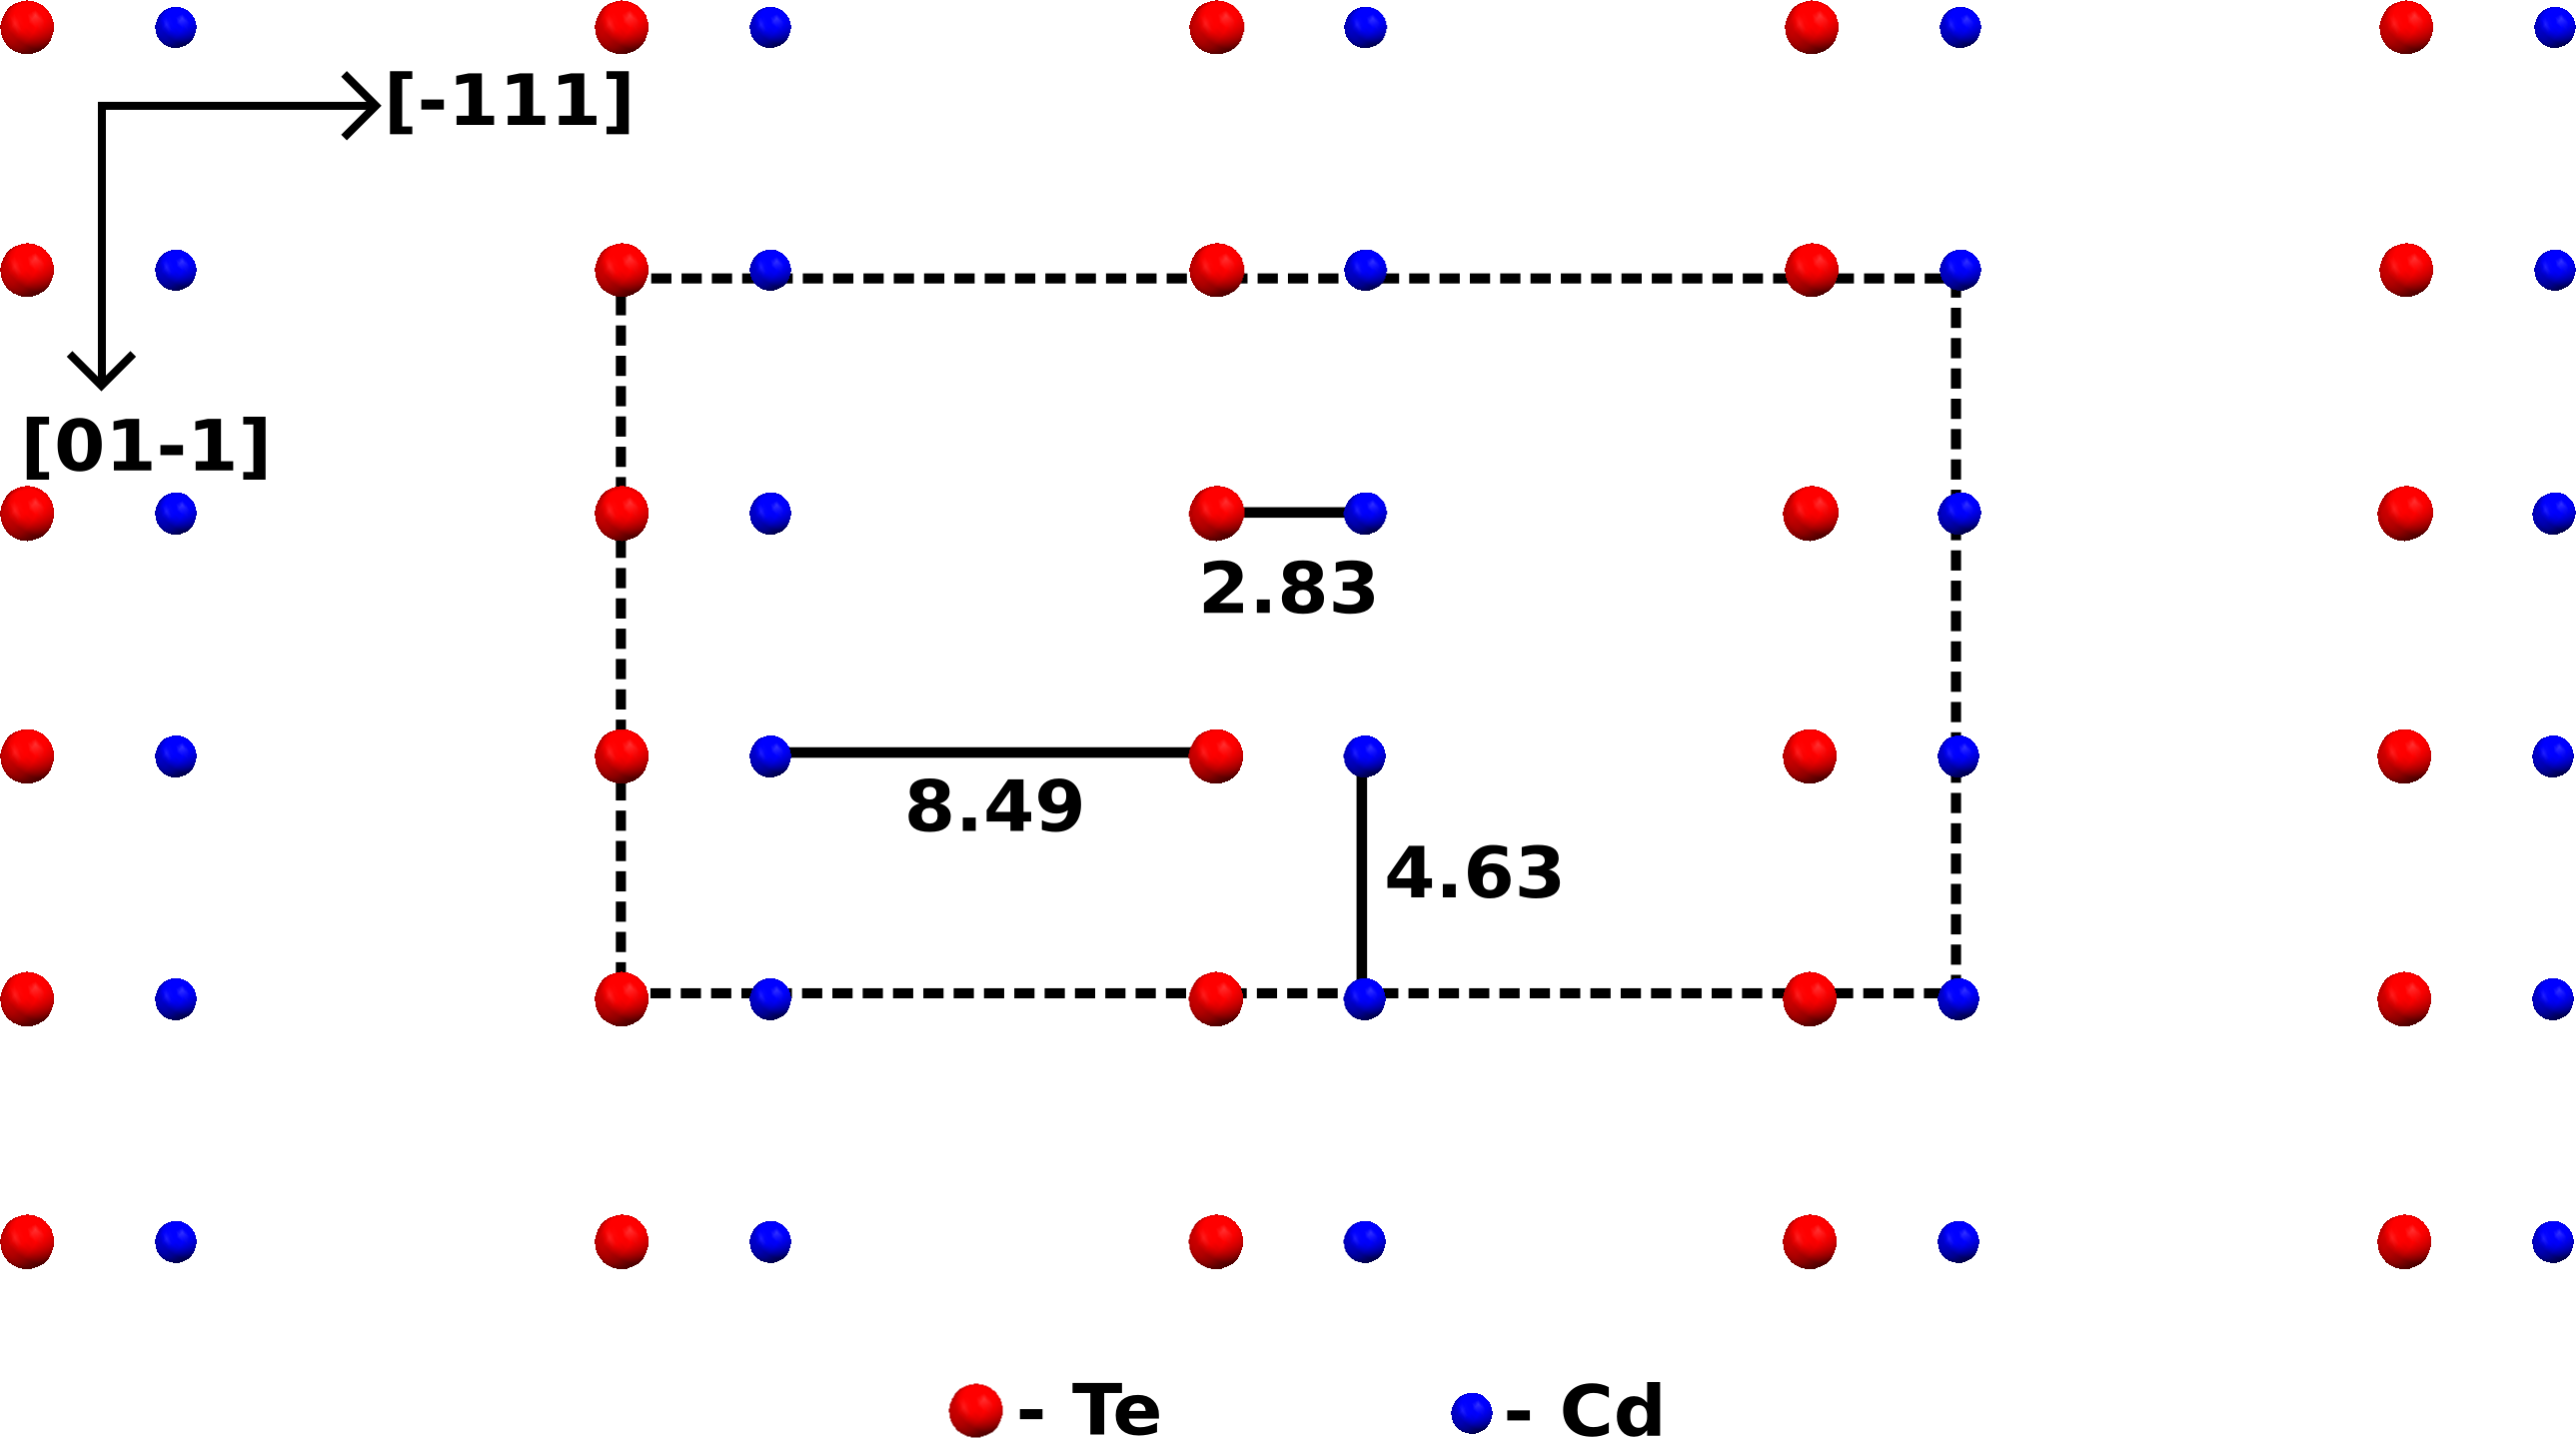
\includegraphics[width=0.8\textwidth]{srtio3_cdte211}
    \caption[Projection of (211) CdTe unit cell on SrTiO\textsubscript{3} surface]{\label{fig:srtio3_cdte211}Schematic of the (211) plane of CdTe with the interplanar dimensions
        labelled in units of angstroms. The area outlined by the dashed lines is used in
        subsequent figures to demonstrate how this structure fits to (100) SrTiO\textsubscript{3} surface
        reconstructions. The Miller indices shown correspond to the crystallographic
        orientation of the (211) CdTe plane.}
\end{figure}
\begin{figure}
    \centering
    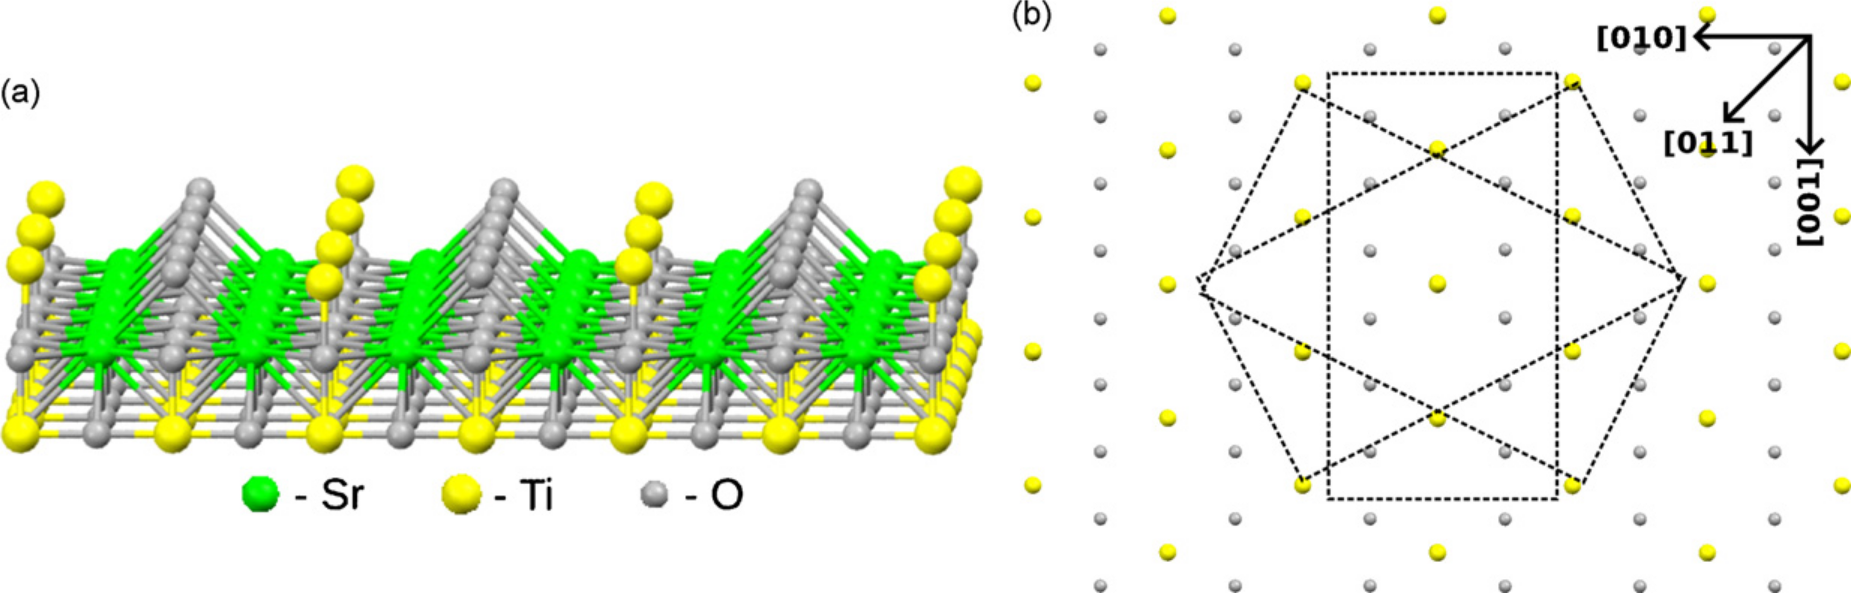
\includegraphics[width=\textwidth]{srtio3_c4x2}
    \caption[CdTe on c(4$\times$2) SrTiO\textsubscript{3} surface]{\label{fig:srtio3_c4x2}(a) Schematic showing the surface of the (100) SrTiO\textsubscript{3} with a c($4\times2$) surface reconstruction. (b) Schematic showing the uppermost layer of the reconstruction with the dashed lines being used to illustrate the closest geometrical fits of the (211) CdTe plane to this surface. The three orientations shown give rise to six grain orientations as a 180\degree~rotation of the (211) plane yields a different grain structure. This is a consequence of the fact that the single crystal (111) CdTe pole figure for a [211] film is one-fold symmetric (see Fig. 3b). Six other grain structures arise from a domain structure in the substrate surface reconstruction that would be schematically represented by a 90\degree~rotation of Fig. 8b. The Miller indices shown in the top right corner of the figure correspond to the crystallographic orientation of the underlying bulk (100) SrTiO\textsubscript{3} substrate.}
\end{figure}
Assuming that the orientational relationships between CdTe
and the surface reconstructions shown in Figs. 8 and 9 are adhered
to then it becomes possible to experimentally predict the surface
reconstruction undergone by the substrates presented in this
work. It should be noted from Fig. 8b that the c($4\times2$)
reconstruction is characterized by (211) CdTe grain alignment
along the substrate’s [010] and [001] directions. Fig. 4b clearly
shows that this is not the case, ruling out this reconstruction for the
work presented here. It does not, however, rule out the possibility
of [211] CdTe grain growth if a film were deposited on such a
reconstruction. The c($6\times2$) reconstruction, on the other hand,
requires grain growth along the substrate’s [011] and [0$\overline{1}$1]
directions, consistent with the X-ray data. While we have no direct
evidence that the c($6\times2$) surface reconstruction formed, it is of
note that the anneal conditions used elsewhere\cite{Jiang1996} to obtain this
reconstruction are similar to those used here. While it should be
understood that predicting a film-substrate orientational relationship solely on the basis of a geometrical fit is somewhat naive, it is well established that this scenario occurs more often than not.
\begin{figure}
    \centering
    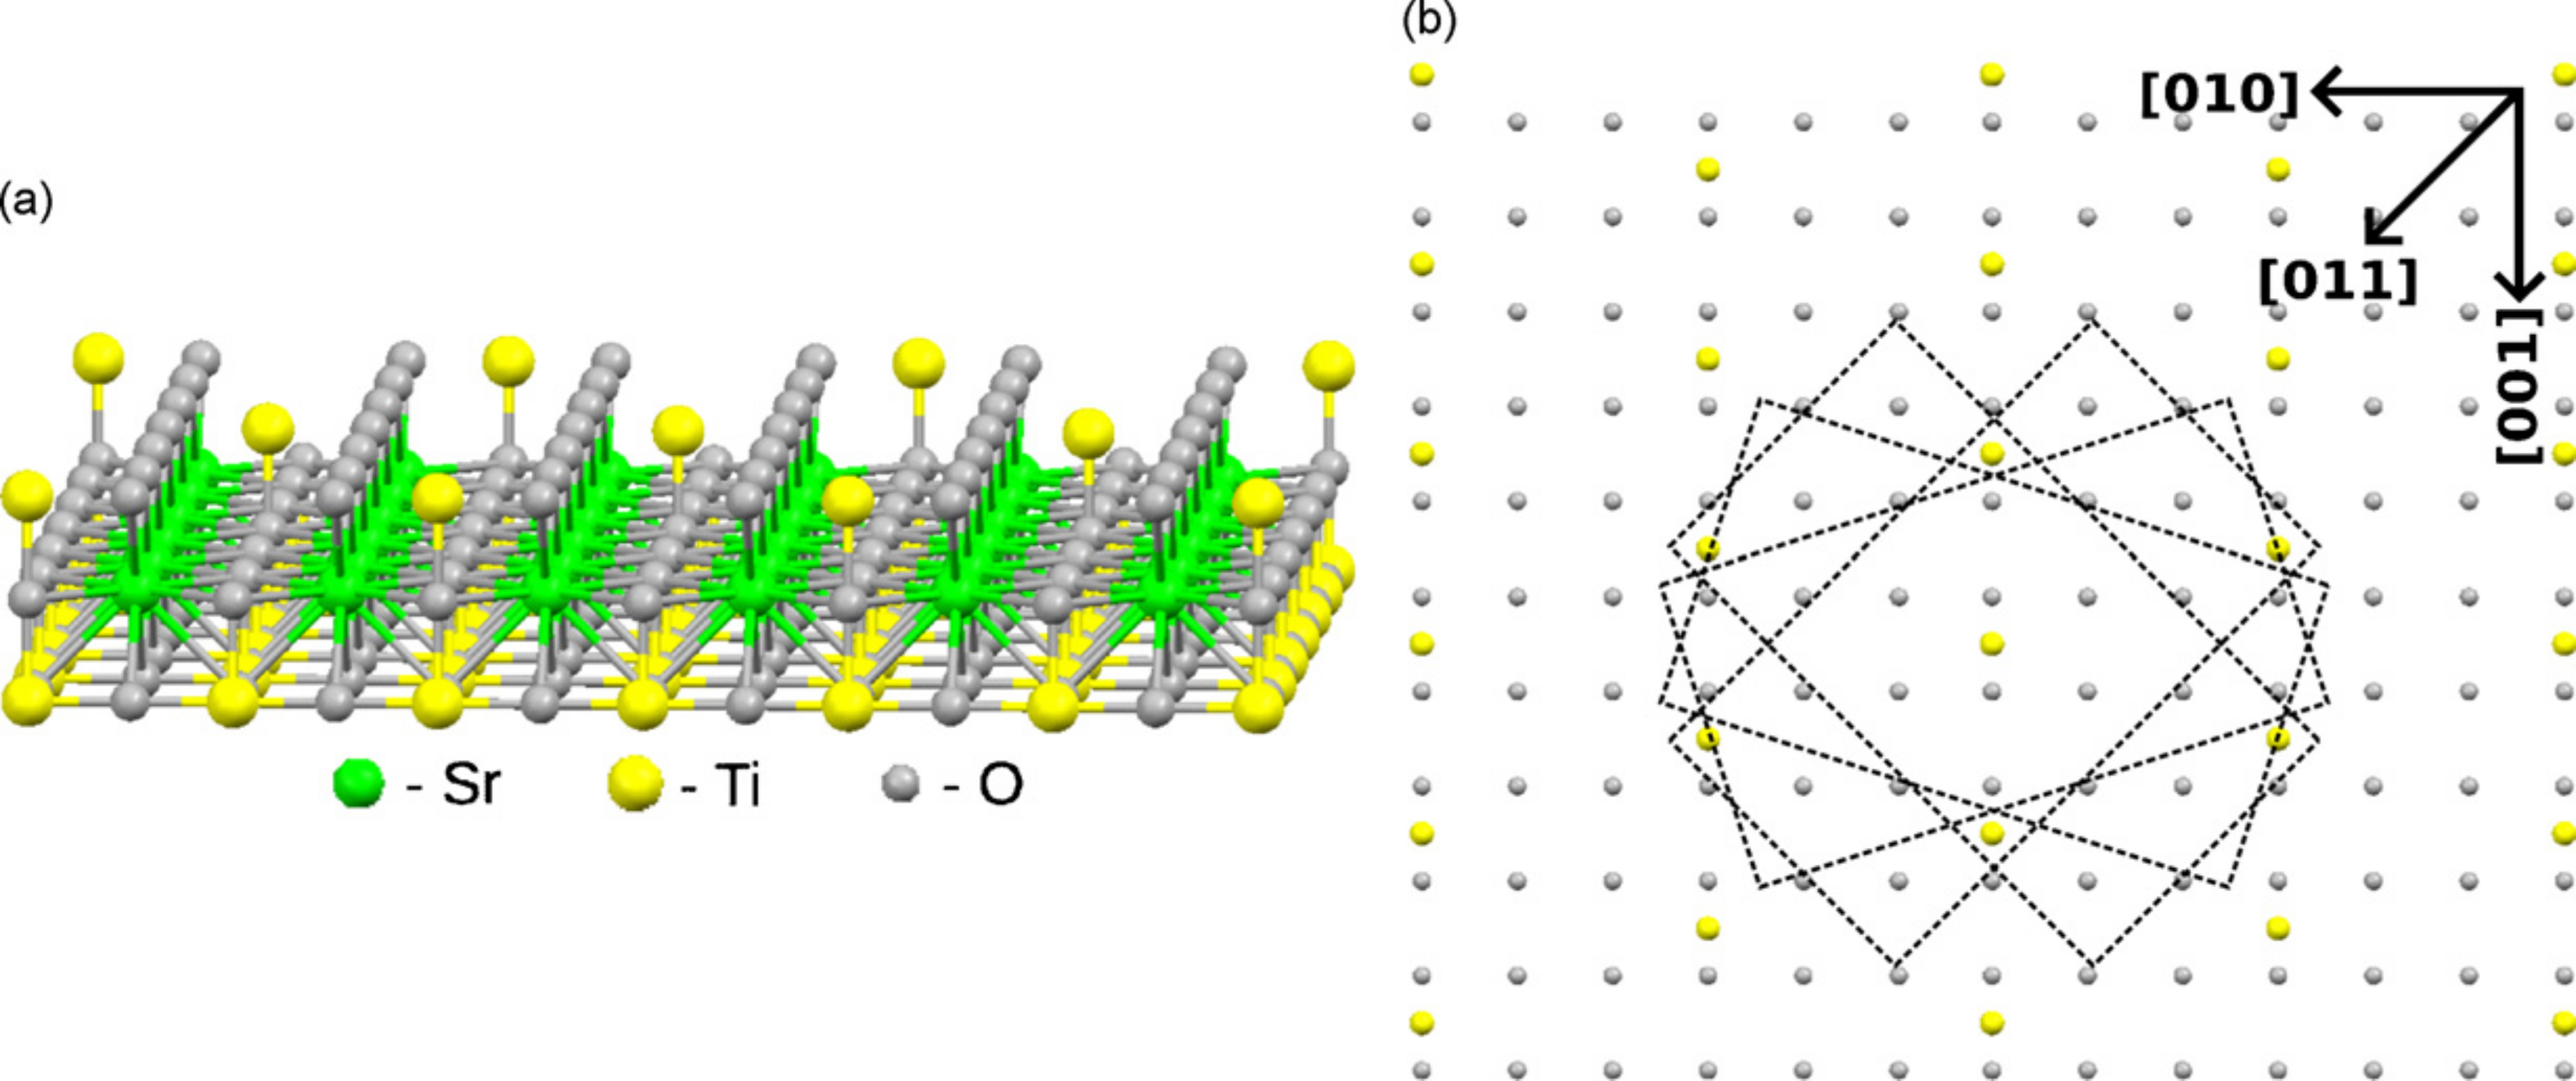
\includegraphics[width=\textwidth]{srtio3_c6x2}
    \caption[CdTe on c(6$\times$2) SrTiO\textsubscript{3} surface]{\label{fig:srtio3_c6x2}(a) Schematic showing the surface of the (100) SrTiO\textsubscript{3} with a c($6\times2$) surface reconstruction. (b) Schematic showing the uppermost layer of the reconstruction with the
        dashed lines being used to illustrate the closest geometrical fits of the (211) CdTe plane to this surface. The four orientations shown give rise to eight grain orientations as a
        180\degree~rotation of the (211) plane yields a different grain structure. Eight other grain structures arise from a domain structure in the substrate surface reconstruction that
        would be schematically represented by a 90\degree~rotation of Fig. 8b. Of these eight grains only four represent unique solutions as the grains forming along the [011] and [01$\overline{1}$]
        directions rotate into each other. The Miller indices shown in the top right corner of the figure correspond to the crystallographic orientation of the underlying bulk (100)
        SrTiO\textsubscript{3} substrate.}
\end{figure}

Even though both the [211] oriented films show pole figure
peaks in similar positions, the relative intensities of the peaks are
quite different. This is most easily seen by examining the
innermost ring of the pole figure where each of the twelve peaks
corresponds to a unique grain orientation. For both samples the
peaks on one side of the ring show greater intensities than on the
other. This effect, however, is much more pronounced for the pole
figure shown in Fig. 4c. Here, the ratio of the integrated intensities
between the largest and smallest peak in the ring is 22 compared to
4 for the pole figure shown in Fig. 4b. The fact that the terrace
width is approximately four times smaller for the film that shows
the most pole figure anisotropy suggests that the step edges
promote this preferential grain alignment. Consistent with this
explanation is the fact that the highest intensity peaks correspond
to the CdTe grain orientation having its [111] in-plane direction
normal to the step. The larger grain sizes exhibited by the surface
with smaller terraces are also expected within this scenario. This is
a simple consequence of the fact that, in the early stages of film
growth, there are more similarly oriented grains that are able to
merge into a single larger grain as is expected for an island growth
mechanism. With a sizeable effect being observed between the two
reconstructed surfaces having a miscut difference of only 0.358, the
potential exists to amplify this effect using a substrate with a
significantly larger miscut.
\section{Implications for Symmetry and Energy at Epitaxial Surfaces}
While the results presented here don't explicitly improve the growth of the CdTe thin films, they do add to the understanding of the role of the interface in epitaxy. In all the cases presented here, the substrate used for epitaxial growth has a nominal orientation of (100), with very small miscut of less than 1\degree. Despite a fixed orientation for the substrate, the thin surface net presented to the epitaxial thin film dominates the nucleation and growth orientation. These results show that it is possible to leverage high temperature surface reconstructions in order to completely transform a given substrate. If a reconstruction can be created at high temperature and then locked-in at the growth temperature substrates that don't immediately appear to be an epitaxial match can end up presenting an ideal template for growth. The additional symmetry breaking that is available for offcut substrates can widen the range of acceptable substrates, by triggering a step-flow growth mode suppressing unwanted orientations.

For this type of surface net epitaxy to yield the most benefit, surface science research must investigate the zoo of surface reconstructions possible on the commercially available complex oxides. Many of the higher element complex oxides (YAG, YSZ, GGG etc.) have little to no literature examining their surface reconstructions or their behaviour when miscut. Phase diagrams of such surfaces would be highly beneficial in predicting good matches for epitaxy.